\section{Machine Learning Basics}
What's a \textbf{machine learning algorithm}? Mitchell (1997) provides the following definition: 

\begin{displayquote}
    "\textit{A computer program is said to learn from experience E with respect to some class of tasks T and performance measure P, if its performance at tasks T, as measured by P, improves with experience E."}
\end{displayquote}

A machine learning \textbf{task} is usually described in terms of how the machine should process an example, which is a collection of features that have been quantitatively measured from some object or event that we want the machine learning system to process. There are several different tasks that can be involved in machine learning, the following two are the most important:
\begin{itemize}
    \item \textbf{Classification}: the computer program is asked to specify which of \textit{k} categories some input belongs to. The learning algorithm is asked to produce a function $f : \mathbb{R}^n \to \{1,...,k\}$ which assigns an input to a category; in some cases, the function $f$ outputs a probability distribution over the classes.
    \item \textbf{Regression}: the computer program is asked to predict a numerical value given some input. The learning algorithm is asked to produce a function $f : \mathbb{R}^n \to \mathbb{R}$.
\end{itemize}
Other typical machine learning tasks are: \textit{denoising}, \textit{density estimation}, \textit{structured output}, \textit{anomaly detection} etc. 

\subsection{Example: Linear Regression}
As the name implies, the linear regression algorithm solves a regression task. More precisely, the algorithm should take a vector $\textbf{x} \in \mathbb{R}^n$ as input and predict the value of a scalar $y \in \mathbb{R}$ as its output. The output of linear regression is a linear function of the output. 
Let $\hat{y}$ be the value predicted for $y$; we define the output to be:
\begin{equation}
    \hat{y} = \textbf{w}^T\textbf{x}
\end{equation}
 where $\textbf{w}\in \mathbb{R}$ is a vector of parameters that we can think of as a set of weights that determine how each feature contributes to the prediction. So we have just defined the task T, now we need a performance measure P to understand how good is our algorithm.
 One option is to compute the \textbf{mean squared error} (\textbf{MSE}) on a test set, which is given by:
\begin{equation}
     \textbf{MSE}_{test} = \frac{1}{m}\sum_{\substack{i}}(\textbf{$\hat{y}$}^{(test)}-y^{(test)})^{2}_{i} 
\end{equation}
In other words, this metric measures the average of the squares of the errors, which is the average squared difference between the estimated values and the actual value. We can denote that the error increases whenever the Euclidean distance between the predictions and the target increases. To make a machine learning algorithm, we have to design an algorithm that it's able to improve the weight's vector $\textbf{w}$ in a way that reduces the MSE when the algorithm is allowed to see new train examples, gaining experience. On intuitive way to do it is to minimize the MSE on the training set, for example by putting the gradient equal to 0.

The term \textbf{linear regression} is often used to refer to a slightly more sophisticated model, which is the following:
\begin{equation}
    \hat{y} = \textbf{w}^T\textbf{x}+b
\end{equation}
This model is still a line, but it doesn't need to pass through the origin.

\vspace{0.5cm}
\begin{center}
    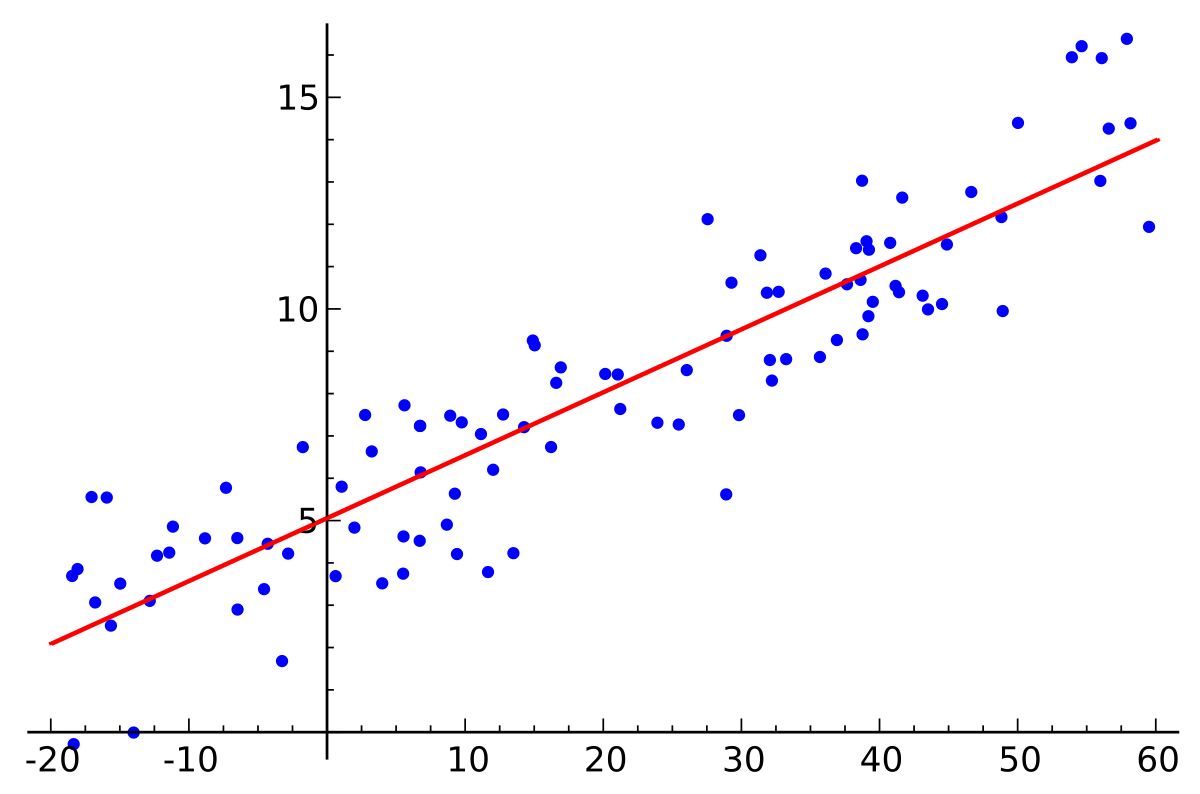
\includegraphics[width=0.45\textwidth]{images_0/linearegre.png}    
\end{center}

The intercept term $b$ is often called the \textbf{bias} parameter, given the fact that the output of the transformation is biased towards $b$ in absence of any input.

\subsection{Capacity, Overfitting and Underfitting}
The central challenge of any machine learning algorithm is to be able to perform well on unseen inputs. The ability to perform well on previously unobserved input is called \textbf{generalization}.

Typically, we training a machine learning algorithm, we can compute some error measure over some training set, the \textbf{training error}, trying to reduce this error; this is simply an optimization problem. What separates machine learning from optimization is that we want to minimize also the \textbf{generalization error}, also called \textbf{test error}. The generalization error is defined as \textit{the expected value of the error on a new input}. When tuning the weights of a machine learning algorithm, we try to find those parameters that minimize the training error, so the test error will generally be greater or equal than the train error. The factors the determine how well an algorithm performs are its ability to:
\begin{itemize}
    \item make the training error small;
    \item make the gap between training and test error small.
\end{itemize}
This correspond to two of the central challenges of machine learning: \textbf{underfitting} and \textbf{overfitting}. The first one occurs when our algorithm is not able to obtain a sufficiently small error value on the training set; the latter occurs when the gap between training and test error is too large.

We can control wheter a model is more likely to overfit or underfit by altering its \textbf{capacity}, which can be informally defined as the ability to fit a wide variety of functions. Models with low capacity may struggle to fit the training set, while models with high capacity tend to overfit by memorizing properties of the training set that do not serve on the test set. One way to control the capacity is by choosing the appropriate \textbf{hypothesis space}, the set of functions that can be chosen by the learning algorithm as being the solution. For example, for linear regression we can generalize to include also polynomials of higher degree, this will increase the model capacity. In general, machine learning algorithms will perform well when their capacity is appropriate to the true complexity of the task that they need to perform and the size of the training data they are provided with.